\documentclass[a4paper,12pt]{article}
\usepackage{graphicx, float, fancyheadings, a4wide, makeidx, verbatim,avant,helvet}
\usepackage{}
\pagestyle{fancyplain}
\setlength{\parindent}{0pt}
\setlength{\parskip}{6pt}

\newcommand{\param}[1] {\begin{math} \langle #1 \rangle\end{math} }
%\newcommand{\param}[1] {\verb1<#1>1 }

\title{\sf{WebBrick 6-64, Model WB10B60}\linebreak Internal Testing results \linebreak Version 1.03}
\lhead{\small{WebBrick 6-64 test results}}
\rfoot{\tiny{www.WebBrickSystems.com}}
\lfoot{\tiny{\copyright L.P.Klyne}}

\author{Andy Harris}

\makeindex

\begin{document}

\maketitle

\begin{figure}[H]
\centering

\includegraphics[width=0.2\textwidth]{Images/WebBrickSystems.png}
\end{figure}

\begin{figure}[H]
\centering

\includegraphics[width=0.3\textwidth]{Images/wb_logo.jpg}
\end{figure}

November 2005 Document Version 1.01 - Initial Version

\begin{description}
\item[WebBrick Software Versions 6.0]
\end{description}

\pagebreak

\tableofcontents

\pagebreak

\section{Introduction}

	The WebBrick is effectivily a web enabled programmable logic controller that is designed to control and monitor various elements of 
	home automation.
	
	Logically and physically it is divided into 3 main components:
	

	\begin{itemize}
	
		\item{\textbf{WebServer}}  This component provides a HTTP and UDP interface to the network via a standard RJ45 socket
		
		\item{\textbf{Processor board}}  This component holds the main processor and oscillator along with a switching step down
		supply and various signal conditioning components.
		
		\item{\textbf{IO board}}  This component is split into two sections, the first provides a base for the processor board and all the
		attendant low voltage and intrinsically safe connections.  The section section handles domestic mains via 4 zero volt switching Triac
		circuits and two relays.


	\end{itemize}

	\begin{figure}[H]
	\centering
	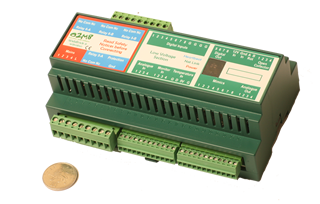
\includegraphics[width=0.7\textwidth]{Images/ObliquePackShotSmallest.png}
	\end{figure}

	
	
\section{General Ratings}

The WebBrick has a full range of connections and operating parameters, those relating to safety are given here:

	\begin{itemize}

		\item{\textbf{Digital Inputs}}  These present 5V DC via weak pull-ups of 4.7K.  Inputs are protected by a CR network
		of 330R and 1uf.  Digital Inputs are triggered by pulling to ground.  Maximum current feed is 5mA.

		\item{\textbf{Analogue Inputs}}  These are high impedance 1M inputs which can accept a 0-5V DC signal.

		\item{\textbf{Dallas 1 Input}}  This provides three connections: 

			\begin{itemize}
		
				\item{} 5V output directly from the switch down power supply maximum 
				current feed is a possible 350mA.
			
				\item{} Data connection, pulled to 5V via 1K, maxium current feed is 5mA
			
				\item{} Ground return
		
			\end{itemize}

		\item{\textbf{Digital Outputs}}  These present a 5V DC signal when in the 'On' state, maximum current feed available is 20mA.
		
		\item{\textbf{Open Collector Outputs}}  These provide a pull to ground output with a maximum sink capacity of 500mA per channel.
		
		\item{\textbf{Analogue Outputs}}  These provide a 0-10V DC signal with a maximum current feed of 50mA per channel
		
		\item{\textbf{Mains outputs}}  These provide 4 mains 240VAC outputs each rated at 4A with an overall capacity of 6.3A aggregated over
		the 4 outputs.
		
		\item{\textbf{Dry Relay Contacts}}  Two double pole changeover relays rated a 4A are provided.  The tracks for these come within
		3mm of the tracks used in the Triac circuits.
		
		\item{\textbf{Mains Protective Ground}}  This provides a safety barrier around the relays and triac drivers and should be
		connected if the WebBrick is used in a mains driven application.
		

	\end{itemize}


	\begin{figure}[H]
	\centering
	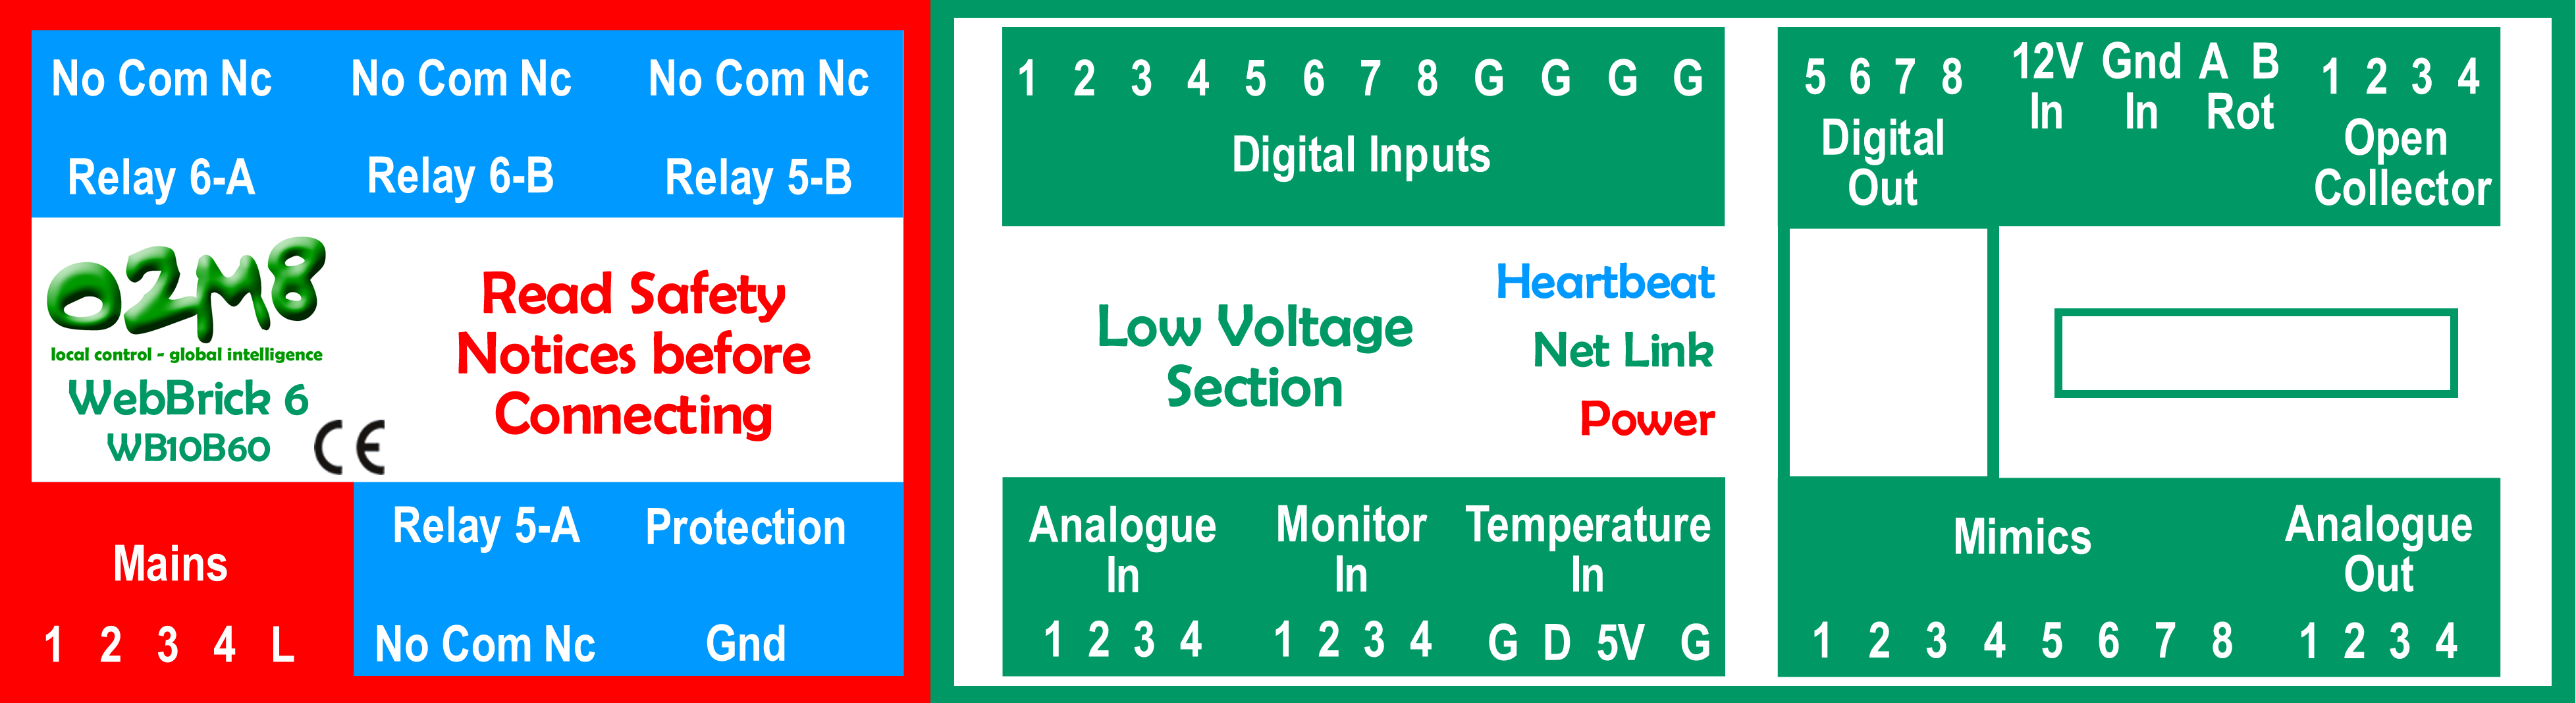
\includegraphics[width=0.7\textwidth]{Images/TopCoverAlt3.png}
	\end{figure}



\section{Full Mains Load Testing}

Two WebBricks were tested at full rated load of 6.3A over three outputs.  The load was provided by 3off 500W halogen lamps.  Testing was conducted in 
an ambient temperature of 21 Deg C to 26 Deg C with a test duration of 2 hours per test.

\subsection{Bare board test}

The WebBricks were tested with the enclosures removed.

	\subsubsection{Results}

	 After two hours the heatsink reached a temperature of 79 Deg C

\subsection{Full product test Horizontal}

	\subsubsection{Results}
	
	 After two hours the heatsink reached a temperature of 104.1 Deg C.  An additional load of 500W was added making the 
	 total load 2kW.  The Heatshink rose to 105 Deg C and the internal fuse blew within 30 seconds.

\subsection{Full product test Vertical}

	\subsubsection{Results}
	
	 After three hours the heatsink reached a temperature of 81 Deg C.  An additional load of 500W was added making the 
	 total load 2kW.  The internal fuse blew within 30 seconds.


\printindex

\end{document}
